\documentclass{article}

\usepackage{amsmath}
\usepackage{amssymb}
\usepackage{tikz}
\usetikzlibrary{shapes,arrows,positioning}
\renewcommand{\thesubsection}{\thesection \space \alph{subsection})}

\title{Planing, Learning and Intelligent Decision Making - Homework 1}
\author{99326 - Sebastião Carvalho, 99331 - Tiago Antunes}
\date{\today}

\begin{document}

\maketitle

\tableofcontents

\section{Question 1}

\subsection{}

First, let's start by showing this problem can be represented as a Markov Chain model. To do this, we need to show it
satisfies the Markov property, that is, the probability of the next state depends only on the current state and not on the
sequence of events that preceded it.

\bigskip

Since the movement of the bot is random, the probability of the bot moving to a certain state depends only on the current document
the bot is in. This means that the bot's movement satisfies the Markov property, and can be represented as a Markov Chain.

\bigskip

Using $\mathcal{X}$ as the state space, $\mathcal{X} = \{ A, B, C\}$, where each state represents its corresponding document.

\bigskip

The transition matrix, $P$, is given by
$
\begin{bmatrix}
    0 & 1 & 0 \\
    0.5 & 0 & 0.5 \\
    1 & 0 & 0
\end{bmatrix}
$.

\bigskip

Where the first row represents the transition probabilities from state A, the second row from state B and the third row from state C.
Each column represents the transition probabilities to state A, B and C, respectively.

\bigskip

The diagram of the Markov chain is given by

\begin{figure}
    \centering
    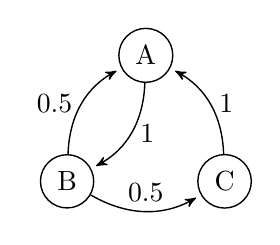
\begin{tikzpicture}[->,>= stealth',shorten >=2pt, line width =0.5 pt ,
node distance=2 cm]
        \node [circle, draw] (A) at (0,0) {A};
        \node [circle, draw] (B) at (-1, -1.6) {B};
        \node [circle, draw] (C) at (1, -1.6) {C};
        \path (A) edge [bend left] node [right] {$1$} (B);
        \path (B) edge [bend left] node [left] {$0.5$} (A);
        \path (B) edge [bend right] node [above] {$0.5$} (C);
        \path (C) edge [bend right] node [right] {$1$} (A);
    \end{tikzpicture}
    \caption{Markov Chain}
    \label{fig: markov_chain}
\end{figure}


\subsection{}

For state A, we have 2 possible paths to reach state A again, $A \rightarrow B \rightarrow A$ and 
$A \rightarrow B \rightarrow C \rightarrow A$. With the transition matrix, we can calculate the probability of each path.

\bigskip

Using $x_t$ to represent the state at time t. 

The probability of the first path is $P(x_1=B|x_0=A) * P(x_2=A|x_1=B) = 1 * 0.5 = 0.5.$

The probability of the second path is $P(x_1=B|x_0=A) * P(x_2=C|x_1=B) * P(x_3=A|x_2=C) = 1 * 0.5 * 1 = 0.5.$


Since the first path takes 2 steps and the second path takes 3 steps, 
$T_{AA} = 0.5 * 2 + 0.5 * 3 = 2.5$.

\bigskip

For state B, we have 2 possible paths to reach state B again, $B \rightarrow A \rightarrow B$ and
$B \rightarrow C \rightarrow A \rightarrow B$. With the transition matrix, we can calculate the probability of each path.

The probability of the first path is $P(x_1=A|x_0=B) * P(x_2=B|x_1=A) = 0.5 * 1 = 0.5.$
The probability of the second path is $P(x_1=C|x_0=B) * P(x_2=A|x_1=C) * P(x_3=B|x_2=A) = 0.5 * 1 * 1 = 0.5.$

Since the first path takes 2 steps and the second path takes 3 steps,
$T_{BB} = 0.5 * 2 + 0.5 * 3 = 2.5$.

\bigskip

For state C, we have infinite possible paths to reach state C again, since the bot can stay transitioning between states A and B indefinitely.

The shortest path is $C \rightarrow A \rightarrow B \rightarrow C$, with 3 steps.
The probability of this path is $P(x_1=A|x_0=C) * P(x_2=B|x_1=A) * P(x_3=C|x_2=B) = 1 * 0.5 * 1 = 0.5$.

The second shortest path is $C \rightarrow A \rightarrow B \rightarrow A \rightarrow B \rightarrow C$, with 5 steps.
The probability of this path is $P(x_1=A|x_0=C) * P(x_2=B|x_1=A) * P(x_3=A|x_2=B) * P(x_4=B|x_3=A) * P(x_5=C|x_4=B) 
= 1 * 1 * 0.5 * 1 * 0.5 = 0.25$.


To calculate the average number of steps, we need to calculate $\sum_{n=1}^{\infty} (2n + 1) / 2^n$, 
where $2n + 1$ is the number of steps and $1/2^n$ is the probability of the path. n represents the number of times we arrive at 
state B.

\bigskip

We can split the sum into two parts, $\sum_{n=1}^{\infty} 2n / 2^n$ and $\sum_{n=1}^{\infty} 1 / 2^n$.

For the first sum, if we take the 2 from the denominator, we get $\sum_{n=1}^{\infty} n / 2^{n}$, which is an Arithmetico-Geometric series.
For an Arithmetico-Geometric series of the form $\sum_{n=1}^{\infty} nq^{n}$, the sum is given by $\frac{q}{(1 - q)^2}$, if $0 < q < 1$.
With this, the first sum is $ 2 * \frac{1/2}{(1 - 1/2)^2} = 2 * \frac{0.5}{0.25} = 4$.

The second sum is a geometric series, with the sum given by $\frac{1}{1 - q} - 1$, if $0 < q < 1$.
With this, the second sum is $\frac{1}{1 - 1/2} - 1 = 2 - 1 = 1$.

\bigskip

With this, the sum of the 2 series is $4 + 1 = 5$, and $T_{CC} = 5$.

\subsection{}

Knowing that $\mu_{x}$ is inversely proportional to $T_{xx}$, we can calculate $\mu_{x}$ for each of the states with the results from above.

\bigskip

$\mu_{A} = 1 / T_{AA} = 1 / 2.5 = 2 / 5 = 0.4$

$\mu_{B} = 1 / T_{BB} = 1 / 2.5 = 2 / 5 = 0.4$

$\mu_{C} = 1 / T_{CC} = 1 / 5 = 0.2$

\bigskip

To get the distribution $\mu$ we must normalize the values calculated previously.

\bigskip

$\mu = \begin{bmatrix} \mu_{A} & \mu_{B} & \mu_{C} \end{bmatrix} / (\mu_{A} + \mu_{B} + \mu_{C}) = \begin{bmatrix} 0.4 & 0.4 & 0.2 \end{bmatrix} / 1 = \begin{bmatrix} 0.4 & 0.4 & 0.2 \end{bmatrix}$

\bigskip

For this distribution to be an invariant of the chain then $\mu_{x} > 0 : x \in \mathcal{X}$, such that 
$\sum_{x \in \mathcal{X}} \mu_{x} = 1$, and $\mu_{x} = \mu_{x}P$, that is $\mu_{x} = \sum_{y \in \mathcal{X}} \mu_{y}P(x | y)$ 
for all $x \in \mathcal{X}$.
The first condition is trivial to verify, all probabilities are higher than 0.
From the second and third conditions we get:

\begin{equation}
    \left\{\begin{array}{@{}l@{}}
        \mu_{A} = \sum_{y \in \mathcal{X}} \mu_{y}P(A | y)\\
        \mu_{B} = \sum_{y \in \mathcal{X}} \mu_{y}P(B | y)\\
        \mu_{C} = \sum_{y \in \mathcal{X}} \mu_{y}P(C | y)\\
        \mu_{A} + \mu_{B} + \mu_{C} = 1\\
    \end{array}\right.\notag
    \Leftrightarrow
    \left\{\begin{array}{@{}l@{}}
        \mu_{A} = \mu_{A} * 0 + \mu_{B} * 0.5 + \mu_{C} * 1\\
        \mu_{B} = \mu_{A} * 1 + \mu_{B} * 0 + \mu_{C} * 0\\
        \mu_{C} = \mu_{A} * 0 + \mu_{B} * 0.5 + \mu_{C} * 0\\
        \mu_{A} + \mu_{B} + \mu_{C} = 1\\
    \end{array}\right.
    \Leftrightarrow
    \left\{\begin{array}{@{}l@{}}
        \mu_{A} = 0.5\mu_{B} + \mu_{C}\\
        \mu_{B} = \mu_{A}\\
        \mu_{C} = 0.5\mu_{B}\\
        \mu_{A} + \mu_{B} + \mu_{C} = 1\\
    \end{array}\right.
\end{equation}

\begin{equation}
    \Leftrightarrow
    \left\{\begin{array}{@{}l@{}}
        \mu_{B} = 2\mu_{C}\\
        \mu_{B} = \mu_{A}\\
        \mu_{C} = 0.5\mu_{B}\\
        \mu_{A} + \mu_{B} + \mu_{C} = 1\\
    \end{array}\right.\notag
    \Leftrightarrow
    \left\{\begin{array}{@{}l@{}}
        \mu_{B} = 2\mu_{C}\\
        \mu_{B} = \mu_{A}\\
        \mu_{C} = 0.5\mu_{B}\\
        2\mu_{C} + 2\mu_{C} + \mu_{C} = 1\\
    \end{array}\right.
    \Leftrightarrow
    \left\{\begin{array}{@{}l@{}}
        \mu_{B} = 2/5\\
        \mu_{A} = 2/5\\
        \mu_{C} = 1/5\\
        \mu_{C} = 1/5\\
    \end{array}\right.
\end{equation}

\bigskip

Which gives us the row vector $\begin{bmatrix} 0.4 & 0.4 & 0.2 \end{bmatrix}$, equal to the distribution obtained above, thus proving that the distribution $\mu$ is invariant of the chain.

\end{document}